\setAuthor{Ardi Loot}
\setRound{lõppvoor}
\setYear{2017}
\setNumber{G 8}
\setDifficulty{9}
\setTopic{Geomeetriline optika}

\prob{Kaamera}
Juku pildistab virmalisi iseehitatud kaameraga, mis koosneb ruudukujulisest
valgustundlikust elemendist küljepikkusega $2h=\SI{2.0}{cm}$ ja kumerläätsest
fookuskaugusega $f=\SI{14}{cm}.$ Jukule ei meeldi, et kaamera on
niivõrd suur ja ta tahab, et kaamera oleks maksimaalselt $L_{m}=\SI{7.0}{cm}$
pikk (kaamera pikkus on kaugus valgustundlikust elemendist välimise läätseni).
Selleks paigaldab ta vana kumerläätse asemel uue kumerläätse fookuskaugusega $f_{2}=\SI{3.0}{cm}$
valgustundlikust elemendist kaugusele $L_{m}.$ Kui suure fookuskaugusega
ja kui kaugele kumerläätsest peaks Juku süsteemi
lisama ühe nõgusläätse, et säiliks kaamera esialgne vaatenurk?

\hint
Tekitagu lõpmatuses asuv objekt läbi kumerläätse ja nõgusläätse vastavalt kujutised $A'$ ja $A$. Kaamera vaatenurk on leitav, vaadates olukorda, kus $A$ asub valgustundliku elemendi ääres. Sellisel juhul on kaamera vaatenurk $A'$ poolt kaetav nurk kumerläätse keskpunktist vaadatuna.

\solu
On selge, et kuna virmalised asuvad kaugel, peab terava kujutise
tekkimiseks olema valgustundlik element esialgse läätse fookuses,
st kaugusel $f=\SI{14}{cm}.$ Kuna läätse keskpunkti läbiv kiir suunda
ei muuda, saame esialgseks vaatenurgaks $2\alpha=2\arctan\left(h/f\right).$

\begin{center}
	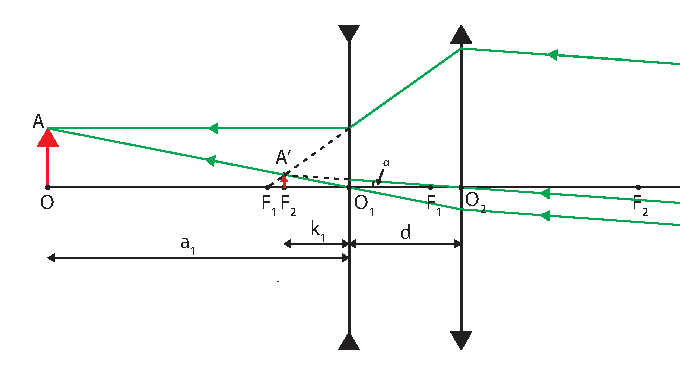
\includegraphics[width=10cm]{2017-v3g-08-skeem__telephoto.pdf}
\end{center}
Joonisel on kujutatud kompaktse kaamera skeem. Vaatleme lihtsuse huvides
olukorda tagurpidi, vaadeldav objekt asub fototundliku elemendi asemel
ning kujutis konstrueeritakse lõpmatuses (kiirte pööratavuse printsiip).
Nõguslääts, mis on paigutatud kaugusele $d$ kumerläätsest, tekitab
objektist $A$ näiva kujutise $A'$. Seda näivat kujutist vaadeldakse
kumerläätsega, mis konstrueerib sellest kujutise lõpmatuses. Kirja
saab panna järgnevad võrrandid:
\begin{eqnarray}
\frac{1}{k_{1}}-\frac{1}{a_{1}} = \frac{1}{f_{1}}, \label{2017-v3g-08-eq:telelens-eq1}\\
k_{1}+d = f_{2},\\
a_{1}+d = L_{m}.
\end{eqnarray}

\noindent Neist esimene määrab nõgusa läätse poolt näiva kujutise asukoha.
Teine võrrand garanteerib, et kumerlääts konstrueerib sellest kujutise
lõpmatuses. Kolmas võrrand tagab, et kogu süsteem oleks kompaktne.
Lisaks eeltoodud võrranditele on vaja säilitada ka esialgse kaamera
vaatenurk. Selleks märkame, et joonisel toodud nurk $\measuredangle A'O_{2}F_{2}=\alpha.$
Seetõttu saame kirja panna:
\begin{equation}
\frac{h'}{f_{2}}=\frac{h}{f},
\end{equation}
\noindent kus $h'$ tähistab kujutise $A'$ kõrgust, mille saame leida
kolmnurkade $OAO_{1}$ ja $F_{2}A'O_{1}$ sarnasusest
\begin{equation}
h'=h\frac{k_{1}}{a_{1}.}\label{2017-v3g-08-eq:telelens-eq2}
\end{equation}

Lahendades võrranditest (\ref{2017-v3g-08-eq:telelens-eq1}) - (\ref{2017-v3g-08-eq:telelens-eq2})
tekkinud süsteemi, saame
\begin{eqnarray*}
f_{1} & = & \frac{f_{2}f(L_{m}-f_{2})}{\left(f-f_{2}\right)^{2}}\approx\SI{1.39}{cm},\\
d & = & \frac{f_{2}(f-L_{m})}{f-f_{2}}\approx\SI{1.91}{cm}.
\end{eqnarray*}

\probeng{Camera}
Juku is photographing northern lights with his self-built camera that consists of a square-shaped photosensitive element with a side length $2h=\SI{2.0}{cm}$ and a convex lens of focal length $f=\SI{14}{cm}.$. Juku does not like that the camera is so big and would prefer it to be maximally with a length $L_{m}=\SI{7.0}{cm}$ (the length of the camera is the distance between the photosensitive element and the outer lens). For that he installs a new convex lens of focal length $f_{2}=\SI{3.0}{cm}$ instead of the old one and he places it at the distance $L_{m}.$ from the photosensitive element. What should be the focal length of an additional concave lens in the system and its distance from the convex lens so that the initial camera’s field of view would be the same?

\hinteng
Let us say that an object in infinity creates images $A'$ and $A$ respectively through the convex lens and the concave lens. The camera’s angle of view is found when observing a situation where $A$ is located at the edge of the photosensitive element. In this case the camera’s angle of view is the angle covered by $A'$ when looking from the center of the convex lens.

\solueng
It is clear that since the northern lights are far away then the photosensitive element has to be in the focal point of the initial lens to create a sharp image, meaning at the distance $f=\SI{14}{cm}.$. Because the ray going through the center of the lens does not change direction we get the initial view angle to be $2\alpha=2\arctan\left(h/f\right)$.
\begin{center}
	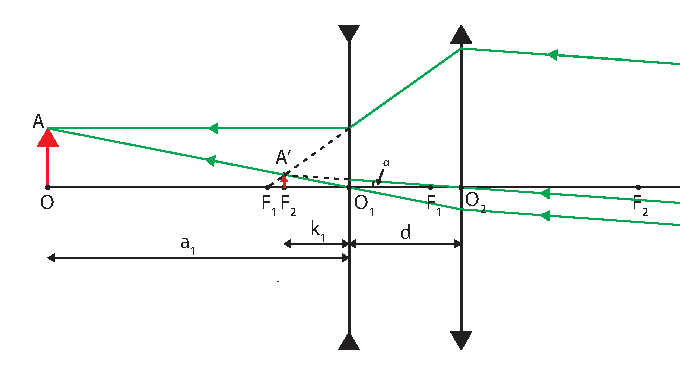
\includegraphics[width=10cm]{2017-v3g-08-skeem__telephoto}
\end{center}
A diagram of a compact camera is pictured in the figure. For simplification let us observe the situation the other way around, the observable object is in place of the photosensitive element and the image is constructed in infinity (principle of reversibility of light). The concave lens that is at the distance $d$ from the convex lens creates a virtual image $A'$ of the object $A$. This virtual image is observed with the convex lens that constructs an image of it in infinity. We can write down the following equations:
\begin{eqnarray}
\frac{1}{k_{1}}-\frac{1}{a_{1}} = \frac{1}{f_{1}}, \label{2017-v3g-08-eq:telelens-eq1}\\
k_{1}+d = f_{2},\\
a_{1}+d = L_{m}.
\end{eqnarray}
With the first of these we find the location of the virtual image created by the concave lens. The second equation guarantees that the convex lens constructs an image of it in infinity. The third equation ensures that the whole system is compact. In addition to the aforementioned equations the initial view angle of the camera also needs to be preserved. For this we notice that the angle given in the figure $\measuredangle A'O_{2}F_{2}=\alpha$. Because of this we can write down:
\begin{equation}
\frac{h'}{f_{2}}=\frac{h}{f},
\end{equation}
where $h'$ is the height of the image $A'$ that we can find from the similarity of triangles $OAO_{1}$ and $F_{2}A'O_{1}$
\begin{equation}
h'=h\frac{k_{1}}{a_{1}.}\label{2017-v3g-08-eq:telelens-eq2}
\end{equation}
Solving the system of equations made from the equations (1) – (5) we get
\begin{eqnarray*}
f_{1} & = & \frac{f_{2}f(L_{m}-f_{2})}{\left(f-f_{2}\right)^{2}}\approx\SI{1.39}{cm},\\
d & = & \frac{f_{2}(f-L_{m})}{f-f_{2}}\approx\SI{1.91}{cm}.
\end{eqnarray*}
\probend